\section{Emilia Sarna}

\subsection{Equasions}
For polynomial of degree $n$: $P(x) = a_{n}x^{n}+a_{n-1}x^{n-1}+\>...\>+a_{1}x+a_{0}$
 Vieta's formulas are: 
\[x_{1}+x_{2}+\cdots\>+x_{n-1}+x_{n}=-\frac{a_{n-1}}{a_{n}}\] 
\[x_{1}x_{2}\cdots\>x_{n-1}x_{n}=-1^{n}\frac{a_{0}}{a_{n}}\]
\[x_{1}x_{2}+x_{1}x_{3}+\cdots\>+x_{n-1}x_{n}=\frac{a_{n-2}}{a_{n}}\]
where $x_{1},x_{2},\cdots\>,x_{n},$ are the roots of this polynomial.

\subsection{Table}
Table~\ref{tab:esarna} represents famous mathematicians and their dates and causes of death.
\begin{table}[htbp]
    \centering
    \begin{tabular}{|c||c|c|}
        \hline
         Name & Date of death & Cause of death \\
         \hline \hline
         John Forbes Nash & 23.05.2015 & Car accident \\
         \hline
         Alan Turing & 7.06.1954 & Cyanide poisoning \\
         \hline
         Stefan Banach & 31.08.1945 & Lung cancer \\
         \hline
         Srinivasa Ramanujan & 26.04.1920 & Hepatic amoebiasis \\
         \hline
         
    \end{tabular}
    \caption{Great mathematicians}
    
    \label{tab:esarna}
\end{table}

\newpage
\subsection{Picture}
A picture of John Venn - English mathematician, logician and philosopher (see~Figure~\ref{fig:Venn}).
\begin{figure}[htbp]
    \centering
    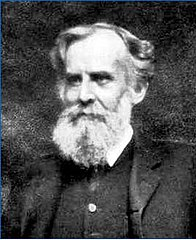
\includegraphics[scale=0.5]{pictures/JVenn.jpg}
    \caption{John Venn (4 August 1834 – 4 April 1923)}
    \label{fig:Venn}
\end{figure}


\subsection{Ordered list}
This is an ordered list of prizes in mathematics:
\begin{enumerate}
    \item Abel Prize
    \item Chern Medal
    \item Fields Medal
    \item Gauss Prize
    \item Nemmers Prize
    \item Balzan Prize
    \item Crafoord Prize
    \item Shaw Prize
\end{enumerate}

\subsection{Unordered list}
This is an unordered list of the same prizes:
\begin{itemize}
    \item [*] Abel Prize
    \item [*] Balzan Prize
    \item [*] Chern Medal
    \item [*] Crafoord Prize
    \item [*] Fields Medal
    \item [*] Gauss Prize
    \item [*] Nemmers Prize
    \item [*] Shaw Prize
\end{itemize}

\subsection{Few paragraphs}
\vspace{0.5cm}\noindent \textbf{\emph{\underline{Mathematics}} is one of the most fascinating fields that you can study.} But beware because it has already led many to madness during countless hours of solving the unsolvable. Many died as well in the pursuit of uncovering mathematics' biggest mysteries \textit{(see~Table~\ref{tab:esarna})}.

However, great devotion comes with a great reward. There is a myriad of prizes and various awards. But there is one that overshadows them all - \underline{mathematical immortality}, fame and glory till the end of our civilization. There is a chance to stand among the great ones: \textbf{\textit{Pythagoras}}, \textbf{\textit{Euclid}} or John Venn \textit{(see~Figure~\ref{fig:Venn})}.